%%%%%%%%%%%%%%%%%%%%%%%%%%%%%%%%%%%%%%
% LaTeX poster template
% Created by Nathaniel Johnston
% August 2009
% http://www.nathanieljohnston.com/2009/08/latex-poster-template/
%%%%%%%%%%%%%%%%%%%%%%%%%%%%%%%%%%%%%%

\documentclass[final]{beamer}
\usepackage[scale=1.24]{beamerposter}
\usepackage{graphicx}			% allows us to import images
\usepackage{bbm,amssymb,mathrsfs}
%\usepackage{natbib}
\usepackage{graphicx,psfrag,dcolumn,amsmath,bm,color}
\usepackage{amssymb}
\usepackage{exscale}
\usepackage{textpos}
\usepackage[tight]{subfigure}
%-----------------------------------------------------------
% Define the column width and poster size
% To set effective sepwid, onecolwid and twocolwid values, first choose how many columns you want and how much separation you want between columns
% The separation I chose is 0.024 and I want 4 columns
% Then set onecolwid to be (1-(4+1)*0.024)/4 = 0.22
% Set twocolwid to be 2*onecolwid + sepwid = 0.464
%-----------------------------------------------------------

\newlength{\sepwid}
\newlength{\onecolwid}
\newlength{\twocolwid}
\newlength{\threecolwid}
\setlength{\paperwidth}{48in}
\setlength{\paperheight}{36in}
\setlength{\sepwid}{0.020\paperwidth}
\setlength{\onecolwid}{0.22\paperwidth}
\setlength{\twocolwid}{0.464\paperwidth}
\setlength{\threecolwid}{0.708\paperwidth}
\setlength{\topmargin}{-0.5in}
\usetheme{confposter}
\usepackage{exscale}

%-----------------------------------------------------------
% The next part fixes a problem with figure numbering. Thanks Nishan!
% When including a figure in your poster, be sure that the commands are typed in the following order:
% \begin{figure}
% \includegraphics[...]{...}
% \caption{...}
% \end{figure}
% That is, put the \caption after the \includegraphics
%-----------------------------------------------------------

\usecaptiontemplate{
\small
\structure{\insertcaptionname~\insertcaptionnumber:}
\insertcaption}

%-----------------------------------------------------------
% Define colours (see beamerthemeconfposter.sty to change these colour definitions)
%-----------------------------------------------------------

\setbeamercolor{block title}{fg=ngreen,bg=white}
\setbeamercolor{block body}{fg=black,bg=white}
\setbeamercolor{block alerted title}{fg=white,bg=dblue!70}
\setbeamercolor{block alerted body}{fg=black,bg=dblue!10}

%-----------------------------------------------------------
% Name and authors of poster/paper/research
%-----------------------------------------------------------

\title{\begin{textblock}{1}(0,-0.1)

\includegraphics[scale=1]{RevisedPlainLogo.jpg}
\end{textblock}Visualization and Causal Inference of the Mexican Drug War}
\author{Valeria Espinosa and Joseph Kelly \vskip0.5ex \small{vespinos@fas.harvard.edu, kelly2@fas.harvard.edu}}
\institute{Statistics Department, Harvard University}%\\[\medskipamount]


%-----------------------------------------------------------
% Start the poster itself
%-----------------------------------------------------------

\begin{document}
\begin{frame}[t]
  \begin{columns}[t]												% the [t] option aligns the column's content at the top
    \begin{column}{\sepwid}\end{column}			% empty spacer column
    \begin{column}{\onecolwid}
			 \vskip-3ex 
 				\begin{block}{Visualize the problem}
					\begin{figure}[htdp]
					    \centering
						\subfigure[2007]{
						    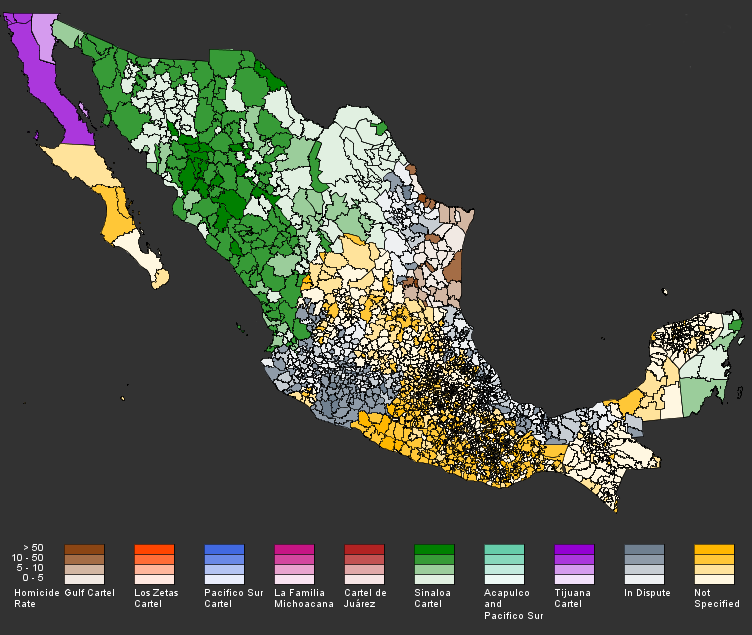
\includegraphics[scale=0.43]{2007.png}
						}
						\subfigure[2010]{
						    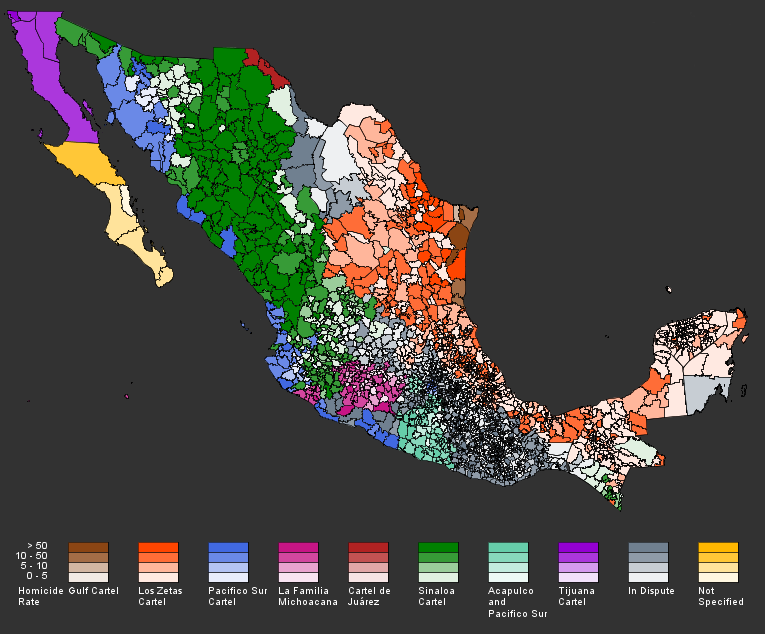
\includegraphics[scale=0.43]{2010.png}
						}
				\end{figure}
	
		%The presidency of Felipe Calder\'{o}n (2006-2012) has been characterized for the war against organized crime, raising many questions regarding security and violence. %We attempt to visualize and analyze homicide rates at the municipality level, and link this to information obtained about the association of drug cartels to municipalities.
		We attempt to answer whether \textbf{homicide rates increase significantly after a military intervention}.
%
%		There are many challenges involved in answering this question. Here, we attempt to point them out and a first try at answering this question. 
%As any good observational study, which mimics a randomized experiment,
 
%The \emph{design} phase was completed without using the outcomes.
		
		
		      \end{block}
      \vskip1ex
      \begin{block}{Estimand}
 Let $Y_i(1)$ denote the homicide rate change in region $i$ from 2006 to one year after receiving a military intervention, and $Y_i(0)$ what it would have been if it hadn't received it (Rubin Causal Model). Our estimand is the average causal effect of the military intervention,  $W$, for the regions that were intervened ($W=1$), $$\tau=\overline{Y}(1)-\overline{Y}(0)=\frac{\sum_{i=1}^{I} Y_i(1)-Y_i(0)}{I}.$$
Let $N_i$ denote the number of municipalities that correspond to region $i$, then 
	$$Y_i(1) = \sum_{j=1}^{N_i}w_{ij}Y_{ij}(1) \textrm{ and } Y_i(0) = \sum_{j=1}^{N_i}w_{ij}Y_{ij}(0),$$	
	$$\textrm{ where }  w_{ij}= \frac{\textrm{Pop}_{ij}}{\textrm{Pop}_{i}} \textrm{ and  }\textrm{Pop}_{i}= \sum_j^{N_i}\textrm{Pop}_{ij}.$$
	However, $Y_i(0)$ and $Y_{ij}(0)$ are missing  $\forall i, j$.
      \end{block}
\begin{block}{Key Assumptions}
		\begin{itemize}
		\item \textbf{SUTVA}
		\begin{itemize}
			\item \textbf{No hidden values of treatments} Broad definition of treatment levels: at least one municipality in the region received an intervention between 2007-2010, or not as reported in \cite{NEXOS} . 
			\item \textbf{No interference between units} Grouped close regions that received an intervention, and their neighboring municipalities to make the ``no interference'' assumption  more reasonable. %For treated regions that are side to side were also assessed in terms of neighboring  geographic situation such as lack of highways connecting them %\url{http://mx.kalipedia.com/kalipediamedia/geografia/media/200805/11/geomexico/20080511klpgeogmx_4_Ges_SCO.png} or big mountains between them, or closeness to where the crops or smuggling routes are \url{http://utopiaguatemala.files.wordpress.com/2011/11/mexico_routes_in_466.gif} (can we find such data?).
	%The last homicide rate that we have corresponds to 2010. That eliminated some of the interventions mentioned in the Nexos paper. 
		\end{itemize}
			\item \textbf{Unconfoundedness} We assume we have all covariates, \textbf{X}, such that given \textbf{X},  treatment assignment is independent of \textbf{Y}.
			 %Unfortunately we didn't get experts to guide most of our decisions. However, we did get to interact with a couple of them and made our covariate choices based on the information received and our understanding of the relevant information. 
			%Our covariates include: location, political party before Calder\'{o}n, income 2006, education and medical information at 2005, percentage of indigenous language speakers, 2006 homicide rate at the municipality level, and GDP, Homicide Rate and Population at the state level.
			\item \textbf{Missing Data} Few treated units had have one missing value (\emph{Doctors per medical unit}). We exactly matched on missingness pattern and Political Party in power in municipality before Calder\'{o}n.
			\item \textbf{Appropriateness of response variable} We assume Y is an adequate measure of violence.	 %Perhaps other crimes should be included			
		\end{itemize}
\end{block}

    \end{column}

    \begin{column}{\sepwid}\end{column}			% empty spacer column
    \begin{column}{\threecolwid}
				 \vskip-3ex 					  % create a three-column-wide column and then we will split it up later
		\begin{block}{Estimation \& Visualization}
			2213 municipalities were included in the initial control pool, and 13 regions (205 municipalities) were considered the treated units. 
			Propensity score matching was used to identify a set of 5 control municipalities that look like each treated ones, and ultimately estimate $Y_{ij}(0)$ and $Y_i(0)$. 
			Let $M_{ij}$ be the number of municipalities matched to the $j$th municipality in region $i$, and $\textrm{PopM}_{ij}=\sum_{k=1}^{M_{ij}}\textrm{PopM}_{ijk}$ is the sum of their populations. Then,
			$$\hat{Y}_{ij}(0) =\sum_{k=1}^{M_{ij}}v_{ijk}Y_{ijk}(0),\textrm{ where } v_{ijk}=\frac{\textrm{PopM}_{ijk}}{\textrm{PopM}_{ij}}.$$
			Therefore,
			$$\hat{Y}_{i}(0) =\sum_{j=1}^{N_i}w_{ij}\hat{Y}_{ij}(0)=\sum_{j=1}^{N_i}w_{ij}\sum_{k=1}^{M_{ij}}v_{ijk}Y_{ijk}(0)=
			\sum_{j=1}^{N_i}\sum_{k=1}^{M_{ij}}\tilde{w}_{ijk}Y_{ijk}(0) \textrm{ with } \tilde{w}_{ijk}=w_{ij}v_{ijk}, $$
			and
			$$\hat{\tau}=\frac{\sum_j Y_j(1)}{J}-\frac{\sum_{j=1}^{J}\hat{Y}_j(0)}{J}=\overline{Y}(1)+\overline{Y}(0) .$$
			We know that $var(\hat{\tau})$ is largest under additivity of potenital outcomes. In that case  $var(\hat{\tau}) =var(\overline{Y}(1))+var(\overline{Y}(0)).$ We use that over estimate to get confidence intervals.% note that this is a case when we wouldn't want to be conservative!!!
			Now, \begin{eqnarray*}
				var(\hat{\overline{Y}}(0))&=&E(var(\hat{\overline{Y}}(0)|Y_i(0) \forall i))+var(E(\hat{\overline{Y}}(0)|Y_i(0) \forall i))
				=E(\sum var(\hat{Y}_i(0))/I)+var(\sum_iY_i(0))/I\\
				&=&E(\frac{\sum_{j,k}w_{ijk}(Y_{ijk}(0)-Y_i(0))^2}{1-\sum_{j,k}w^2_{ijk}})+var(Y(0))/I =\frac{\sum_{i,j,k}w_{ijk}(Y_{ijk}(0)-Y_i(0))^2}{I(1-\sum_{jw}w^2_{ijk})})+S^2(0)/I.\\
			\end{eqnarray*}
			 	Now, $var(\hat{\overline{Y}}(1)) = S^2(1)/I$ because the all $Y_j(1)$ are observed.
				\begin{figure}[htdp]
				    \centering
							
					
					\subfigure[Love plot - balance checks]{
					    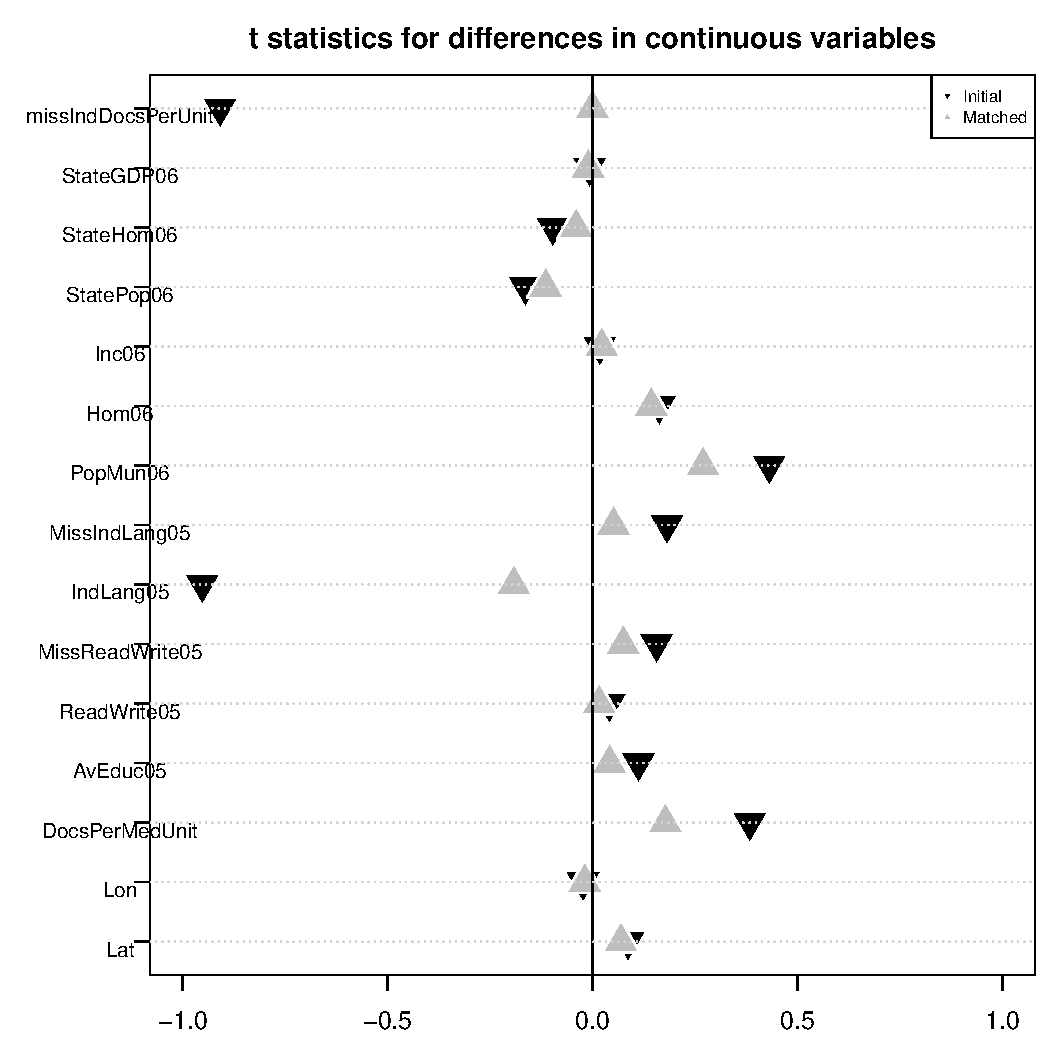
\includegraphics[scale=1]{../Images/FinalLoveplot.pdf}
					}
					\hspace{1cm}
					\subfigure[Interventions and SUTVA]{
					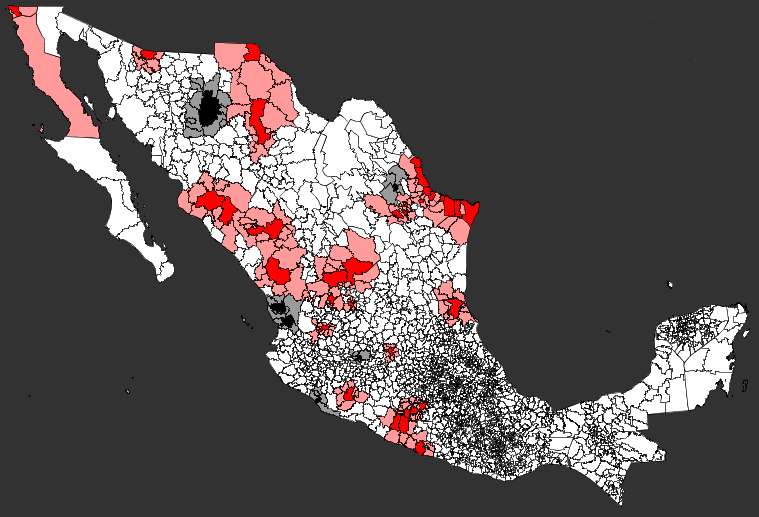
\includegraphics[scale=0.85]{intervened.png}	
					}
					\hspace{1cm}
					\subfigure[Results]{
					   	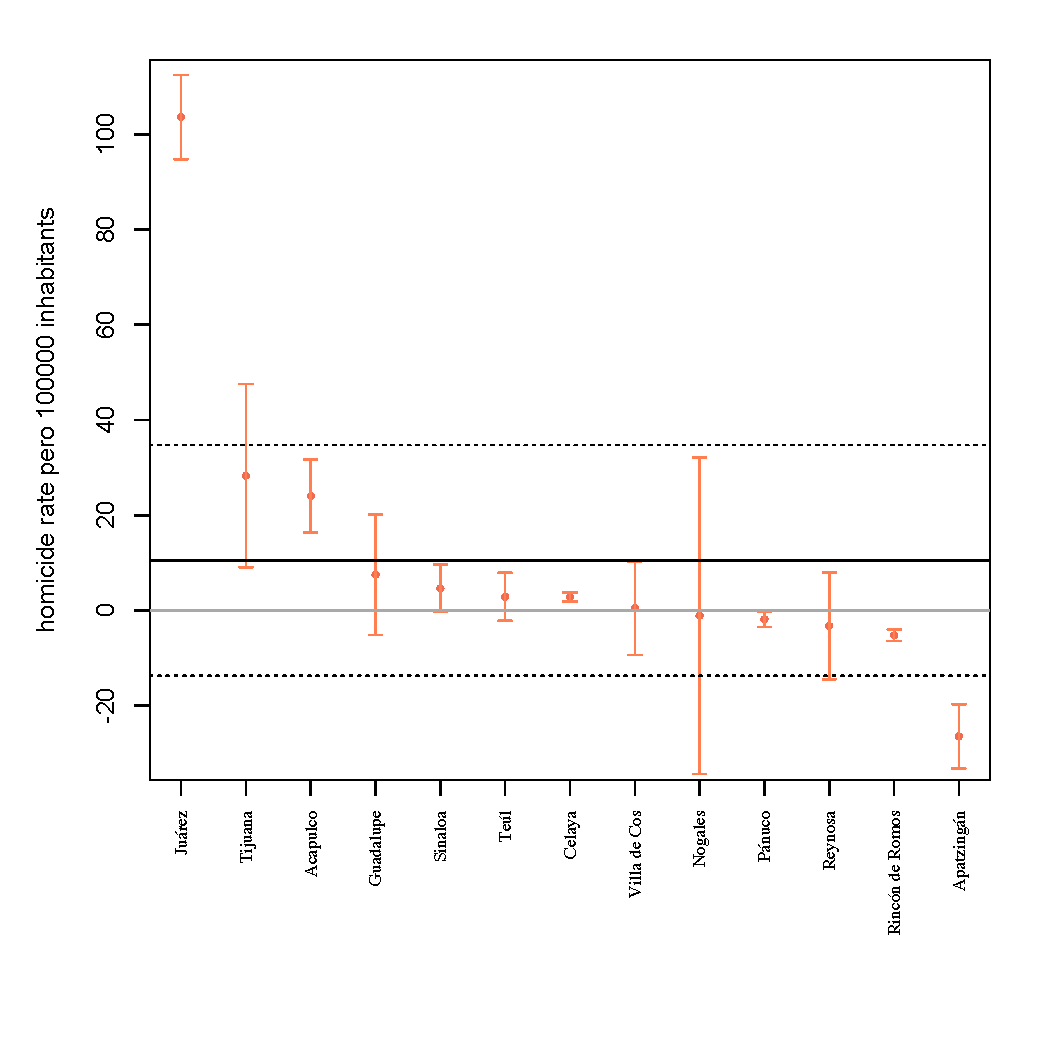
\includegraphics[scale=1.1]{../Images/results.pdf}
					}
			\end{figure}
			
	

				
	 \end{block}
      \begin{columns}[t,totalwidth=\threecolwid]	% split up that three-column-wide column
        \begin{column}{\onecolwid}

          \setbeamercolor{block title}{fg=red,bg=white}%frame color
          \setbeamercolor{block body}{fg=black,bg=white}%body color
          \begin{block}{Results}
				\begin{table}[ht]
				\begin{center}
					\resizebox{25cm}{!}{
				\begin{tabular}{llccc}
				  \hline
				 \textbf{unit}& \textbf{Region}& number of& Date of first & $Y_j(1)-Y_j(0)$ (SD) \\
				 && municipalities& intervention& \\
				  \hline
				4&		  \textbf{Ju\'{a}rez} &  15 & 2009  & 192.99 (79.88) \\ 				
				1&		  \textbf{Tijuana} &   5 & 2008 &20.49  (8.27)\\  
				2&		  \textbf{Nogales} &   5 & 2008 & 11.41  (20.90) \\
				10&	 	  \textbf{Te\'{u}l de Gonz\'{a}lez Ortega} &10 & 2009& 7.32  (4.99) \\
				15&		\textbf{Celaya} &9 & 2009  & 6.74 (1.37) \\ 				
				18&		\textbf{Acapulco} &35 & 2008  & 1.19  (0.77) \\    
				5&		  \textbf{P\'{a}nuco} &  14 & 2007& 0.37  (0.24) \\
				9&		  \textbf{Villa de Cos, Fresnillo}&  18 & 2008& -2.87  (0.34) \\				
				6&		  \textbf{Reynosa} &  24 & 2008 &   -3.49  (1.48) \\
				11&		\textbf{Rinc\'{o}n de Romos} & 8 & 2008& -4.10  (1.05)\\  
				8&		  \textbf{Guadalupe} &  20 & 2009 & -4.27  (0.58) \\  
				12&		\textbf{Sinaloa, Badiraguato, Pueblo Nuevo}&27 & 2007  & -15.84  (0.74) \\ 
				16&		\textbf{Apatzing\'{a}n} &10 & 2007  &-52.81  (5.97) \\ 
				\hline
				\hline 
				&		 \textbf{$\hat{\tau}$}& 205& - &14.61 (23.14)\\
					%   \textbf{7} &   5 & 2010* & \textbf{17} &6 & 2010* \\
					% \textbf{13} &11 & 2010* &  \textbf{14} &9 & 2010* \\ 
					% \textbf{3} &  12 & 2010
				\hline
				\end{tabular}}
				\end{center}
				\caption{}
				\label{tab1}
				\end{table}
          \end{block}
        \end{column}
\begin{column}{\onecolwid}
        %\end{column}
        %\begin{column}{\onecolwid}
          \begin{block}{Key References \& Data Source}
   
            \bibliographystyle{plain}
		        \small{\begin{thebibliography}{99}
				\bibitem{Abadie} Abadie  Synthetic Matching 
				\bibitem{NEXOS} Escalante F, \emph{Homicidios 2008-2009 La muerte tiene permiso}
		        \bibitem{ImbensRubin} Imbens G. \& Rubin D.R., (2012)
				\bibitem{Rubin} Rubin D.R. ,\emph{Matched Sampling for Causal Effects},
				%\bibitem{Valle} Diego Valle visualization
				\bibitem{CIDAC} CIDAC
				\bibitem{INEGI} INEGI
				\bibitem{SMaps} Stratfor Maps
		   \end{thebibliography}}

		      \end{block}
        \end{column}
      \end{columns}
      \vskip2.5ex
    \end{column}
  \begin{column}{\sepwid}\end{column}			% empty spacer column
 \end{columns}
\end{frame}
\end{document}
